\section{Preliminaries}
\subsection{Diffusion models}

\begin{frame}{Diffusion models}

\begin{enumerate}

    \begin{itemize}
        \item Sample $\mathbf{x}_0$ in real data distribution and sample $\mathbf{x}_t$ by
        $$q(\mathbf{x}_t|\mathbf{x}_{t-1}) = \mathcal{N}(\mathbf{x}_t; \sqrt{1-\beta_t}\mathbf{x}_{t-1}, \beta_t\mathbf{I}).$$

        \item For a large $T$, $\{x_t\}_{t\ge T}$ is approximate the Gaussian $\mathcal{N}(0,\mathbf{I})$.
    \end{itemize}
    
    
    \item Reverse process: learn to denoise a Gaussian sample back to a data point in real data distribution
    \begin{itemize}
        \item Try to learn $p_\theta(\mathbf{x}_{t-1}|\mathbf{x}_t) \approx \mathcal{N}(\mathbf{x}_{t-1};\bm{\mu}_\theta(t,\mathbf{x}_t),\bm{\Sigma}_\theta(t,\mathbf{x}_t))$ that best approximates $q(\mathbf{x}_{t-1}|\mathbf{x}_t)$
    \end{itemize}
\end{enumerate}


\end{frame}

\begin{frame}{Diffusion models}
\begin{figure}
    \centering
    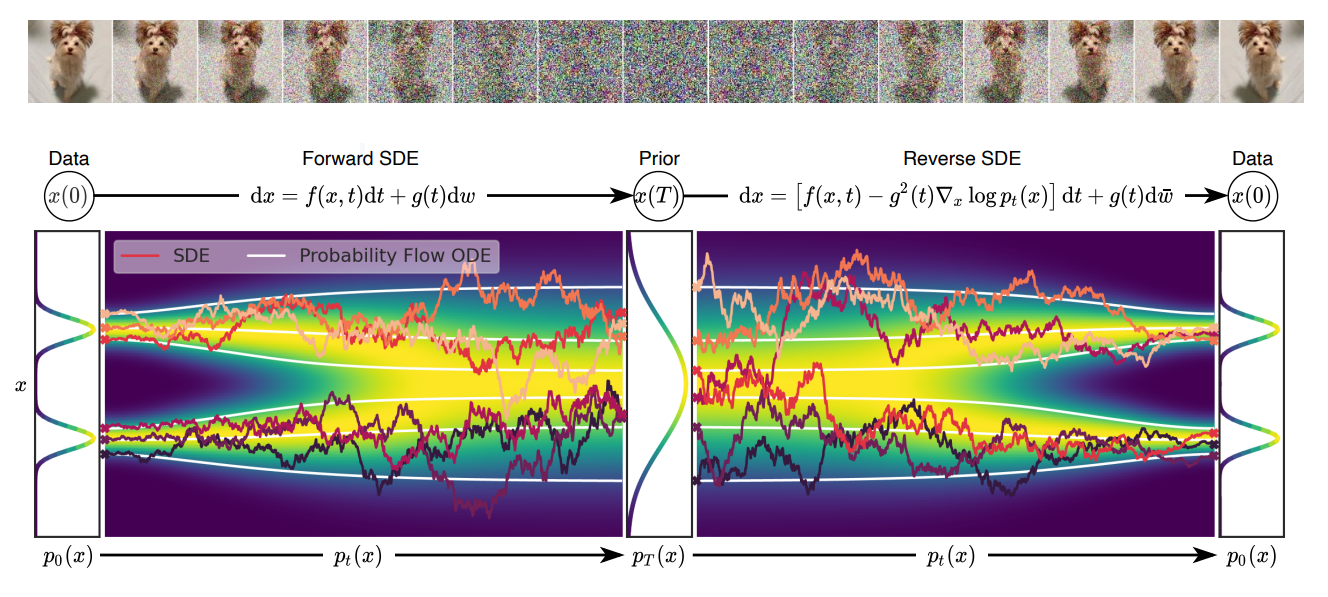
\includegraphics[width=0.8\textwidth]{img/diffusion.png}
    \caption{The Markov chain of forward (reverse) diffusion process of generating a sample by slowly adding (removing) noise. (Image source: Ho et al. 2020 with a few additional annotations)}
    \label{fig:enter-label}
\end{figure}
    
\end{frame}


\subsection{Relevant concepts}

\begin{frame}{Relevant concepts}
    In order to absorb the idea of diffusion models, we have to get familiar to some other theoretical aspects, techniques and tricks
    \begin{enumerate}
        \item Stochastic processes: Markov chains and Wiener process      
        \item Variational Inference
        \item Differential equations
    \end{enumerate}
\end{frame}

\subsection{Watermark types}

\begin{frame}{Common Image Watermark Types}
\begin{itemize}
    \item \textbf{Visible} vs Invisible
    \item Text vs Logo
    % Images each case
\end{itemize}
\end{frame}

\section{Objectives}

\begin{frame}{Watermark removal - Possible approaches}

\begin{enumerate}
    \item \textbf{Denoising}: treat watermarked images as samples that are not in the real distribution 

    \begin{figure}
        \centering
        \includegraphics[width=\textwidth]{img/reconstruct.png}
        \caption{Denoising approach \cite{mousakhan2023anomaly}}
        \label{fig:enter-label}
    \end{figure}
    
    \item \textbf{Inpainting}
    \begin{figure}
        \centering
        \includegraphics[width=\textwidth]{img/inpaint.png}
        \label{fig:enter-label}
    \end{figure}
    % \begin{itemize}
    %     \item Detect - OCR, etc.
    %     \item Select - rectangular or fitted?
    %     \item Remove - adding noise.
    %     \item  Reverse - apply diffusion to inpaint. 
    % \end{itemize}
    
\end{enumerate}
\end{frame}

\begin{frame}{}
\begin{center}
   \textbf{\Huge{Thank you for watching!} }
\end{center}
    
\end{frame}

% \begin{frame}{Watermark removal}
 
% \begin{figure}[!ht]
%   \centering
%   \begin{subfigure}{0.3\textwidth}
%     \centering
%     \includegraphics[width=\textwidth]{img/clean.png}
%     \caption{Clean images}
%   \end{subfigure}
%   \hfill
%   \begin{subfigure}{0.3\textwidth}
%     \centering
%     \includegraphics[width=\textwidth]{img/corrupt_2.png}
%     \caption{Corrupted images}
%   \end{subfigure}
%   \hfill
%   \begin{subfigure}{0.3\textwidth}
%     \centering
%     \includegraphics[width=\textwidth]{img/recon_2.png}
%     \caption{Reconstructed images}
%   \end{subfigure}
%   \caption{Inpainting using Diffusion}
%   \label{fig:1}
% \end{figure}   

% \end{frame}

% \begin{frame}{Watermark removal}
  
%     \begin{figure}
%         \centering
% \includegraphics[width=.8\textwidth]{img/watermarking-removal.png}
%         \caption{Expected result}
%         \label{fig:enter-label}
%     \end{figure}
% \end{frame}

